\subsection{Comparison to Automatic Analysis}

Another approach to detecting induction variables in 
stream programmers involves automatically
recognizing induction variable usage in filter construction. 

The approach of automatic analysis would idiomatically detect 
a variable modified by a statement similar to \texttt{var=var+1}. 
Very few iteration filters, outside of source filters, use induction state 
in this limited capacity. Consider Figure~\ref{fig:transform-after-simple}, where
the induction variable is incremented at each iteration step but resets at 
a threshold value. This pattern is very common in programs that use
induction filters; MPD and FIRBank use this technique to iterate
across a provided array one element per iteration step. 

% \begin{figure}[t]
% {\eightpoint
% \begin{verbatim}
% float->float filter WeightCalc(int n)
% {
%   float[n] window;
%   int windowPos;

%   ...

%   // the input stream is multiplied with the weights
%   work push 2 pop 2
%   {

%     push(pop() * window[windowPos]);
%     push(pop() * window[windowPos]);

%     windowPos++;
%     if(windowPos >= n)
%     {
%       windowPos = 0;
%     }
%   }
% }
% \end{verbatim}
% \caption{MPD filter that multiplies stream values with weights.\protect\label{fig:weight-calc}}}
% \end{figure}


\begin{figure*}[t!]
\centering
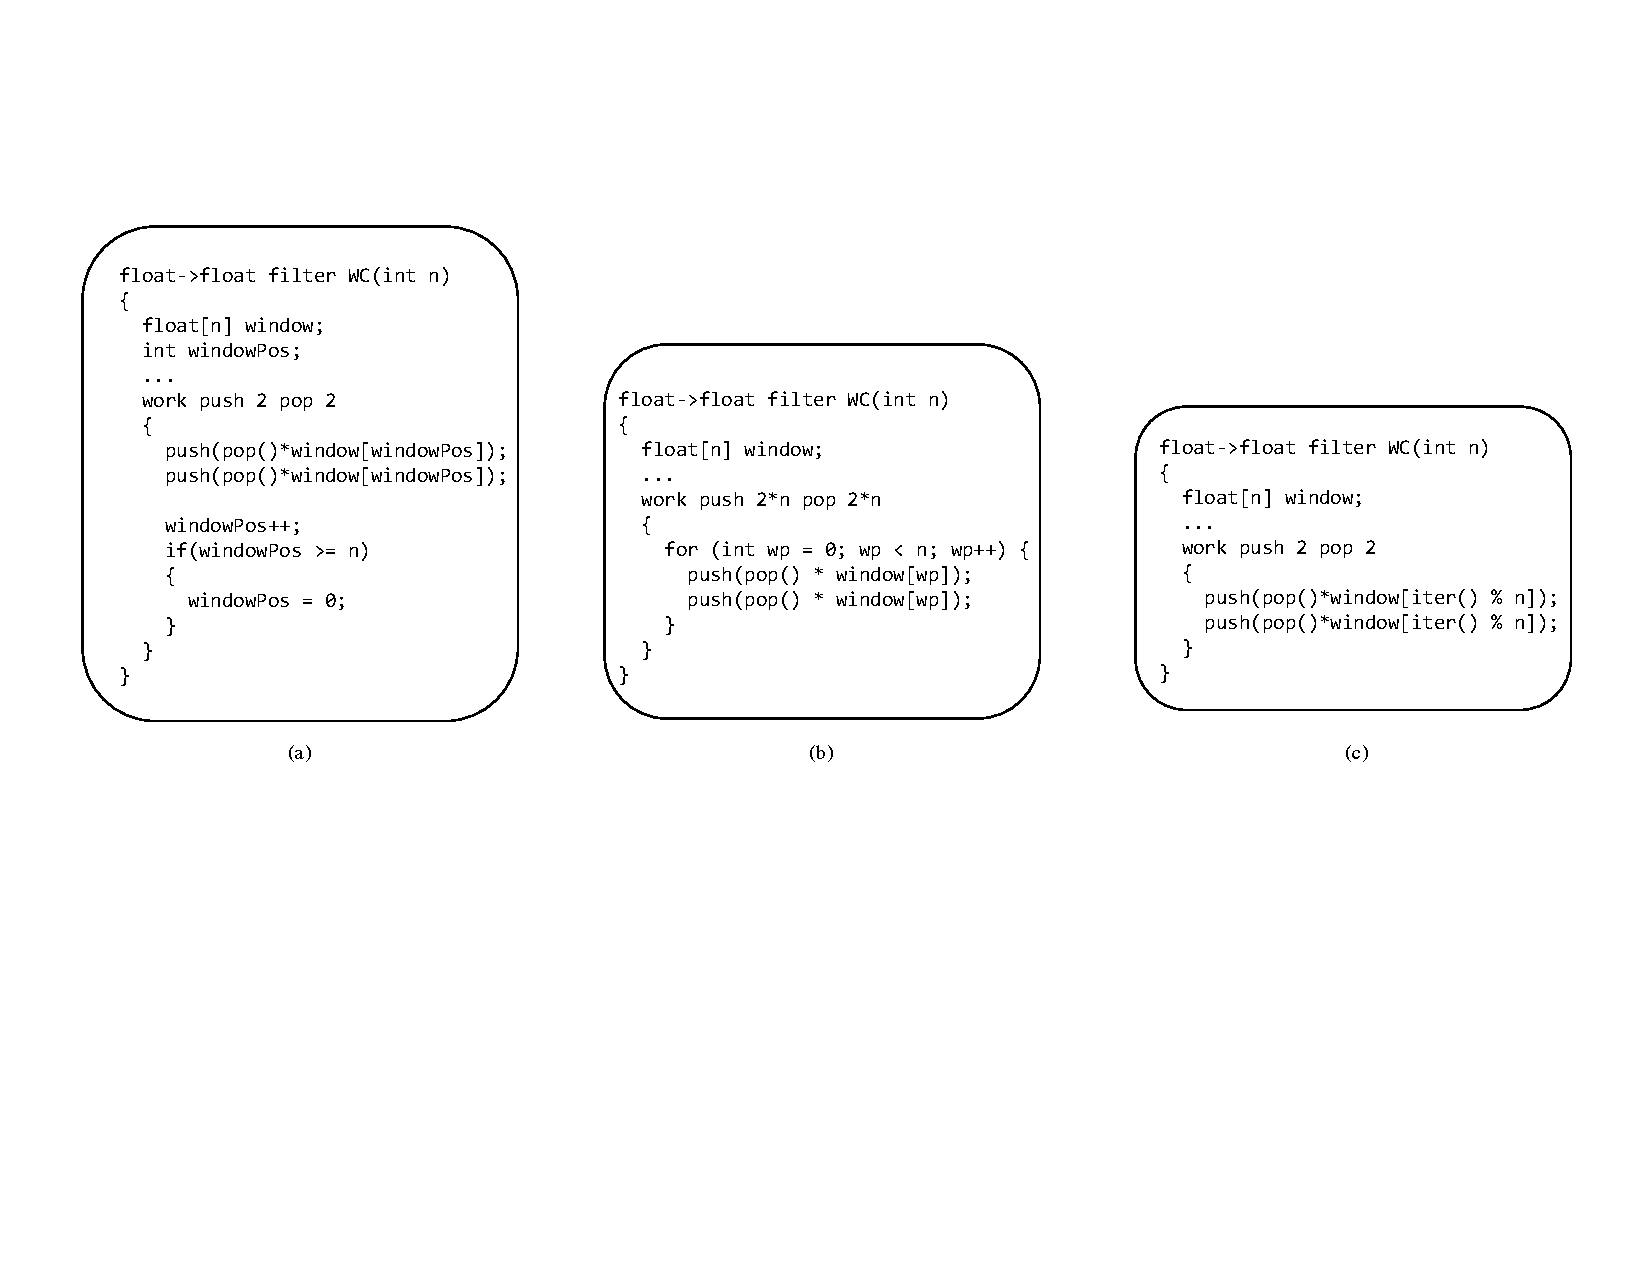
\includegraphics[width=6.5in]{figures/weights-calc-example.pdf}
\caption{Three versions of the weights calculation filter from Medium Pulse Doppler (MPD) (a) is the original filter with explicit induction variable state.  (b) is a coarsened version without state. (c) is a version that utilizes the {\tt iter()} keyword to avoid state.\protect\label{fig:wc-example}}
\end{figure*}


A filter may also have multiple dependent induction variables.  
The stateful filter in Figure~\ref{fig:transform-after-twonested} shows
a filter using nested dependent induction variables.  
Co-induction variables may be constructed to reset the value of 
other induction variables after it reaches a certain value.  

Accordingly, the automatic analysis must be flexible enough to detect 
the induction variable and potentially unpredictable updating statements.  Automatic analysis must be able 
to detect incrementing statements that may not be called on every invocation. The
process of simply detecting and identifying induction variables can 
potentially branch into many cases each needing to be specially implemented.
With the keyword solution, what value the induction variable should take
is left to the user to control, without potentially inhibiting data parallelism
opportunities.

%There may potentially be other special cases that must be defined into the automatic analysis.  Filters may define induction variables that start with and reset to a particular value.  Induction variables may increment by a different value other than one at each execution step.  Co-induction variables may be constructed to reset the value of other induction variables after reaching a certain value.  The different uses of induction variables may be difficult to assess.  Though the methods of using induction variables as illustrated in Figures~\ref{fig:wc-example} and~\ref{fig:transform-after-twonested} encompass many of the common use cases in the benchmark suite, slight variations in the implementation to the pattern may prevent the induction variable from being detected.

% Automatic recognition is fairly inflexible in detecting induction variable state.  The process would restrict data parallelism opportunities to only the filters that fit the implemented templates.  We instead elect to provide the user with the flexibility of defining their own derived induction values.  

It may also be difficult to detect how the induction value will be
updated. The keyword solution has the added benefit of only maintaining
a single value that is predictable in its updates. The value that the 
keyword returns is simply the number of times the filter has been 
invoked. This value is always incremented by one at the end of every work call.

%Furthermore, the approach of automatic analysis does little to
%encourage programming with parallelism in mind. On inspection, user
%written code will still maintain state, which actively inhibits data
%parallelism opportunities. In introducing a language construct, user
%written code appears to eliminate explicitly kept state. This approach
%encourages users to knowingly write code that actively exploits
%data parallelism.
